\chapter{Threat Model}

Security as part of a software project is nowadays an element that should no longer be neglected. When security is considered from the beginning of a project, it is much easier to keep pace of the evolving threat landscape, quickly derive implications in case of an emerging vulnerability and adapt the project where necessary. Another benefit is the significantly shorter time to react as identifying the project's exposure is faster and easier with a constantly kept up-to-date threat model.

Writing secure software starts with the awareness of the various threats a project might exposed to. This includes applications, interfaces, hardware and users, where potential vulnerabilities can impact the reliability and integrity of a system. If the developer team sticks to the practice of continually updating the threat model and implementing security features as part of each deployment, security can actually become a fun topic and an imporant feature of the project.

\section{STRIDE}

For KubeWatch we define our threat model based on the STRIDE model.
\begin{itemize}
    \item [{\bfseries S}]poofing (Authenticity)
    \item [{\bfseries T}]ampering (Integrity)
    \item [{\bfseries R}]epudiation (Non-Repudiation)
    \item [{\bfseries I}]nformation disclosure (Confidentiality)
    \item [{\bfseries D}]enial of Service ( Availability)
    \item [{\bfseries E}]levation of privilege (Authorization)
\end{itemize}


\section{Architecture and Trusted Boundaries}

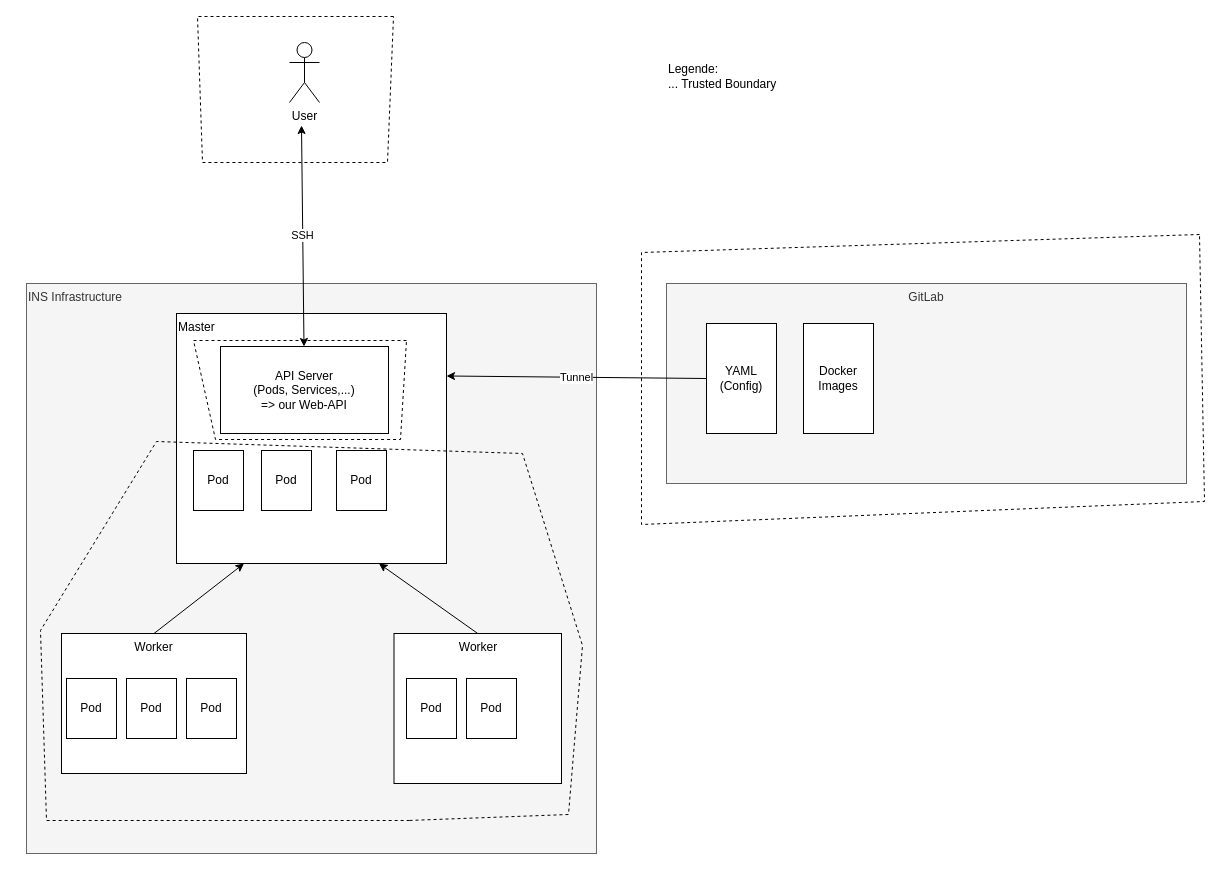
\includegraphics[height=12cm]{resources/architecture_threat_model.png}


\section{Threat Identification}

\begin{tabular*}{\textwidth}{p{2.1cm} p{1.8cm} p{3cm} p{2cm} p{3.5cm}}
    \textbf{Component} & \textbf{Category} & \textbf{Threats} & \textbf{Risk} & \textbf{Mitigation} \\
    \hline
    User                & D, E & Worm & Low & \\
                        & I & Keylogger & Low & \\
                        & & Residual risk & Low & \\
    \hline
    Interface User/Master   & I, T & Man-in-the-middle & Medium & \\
                            & I, T & SQL Injection & Medium & Input validation \\
                            & & & & Patch Services \\
    \hline
    API server          & D & Denial of Service & Medium & CPU limitation \\
                        & & & & Alerts \\
                        & & Service vulnerability (later) & & \\
    \hline
    K8s Cluster             & D & Hardware failure & Low & Keep backups of K8s configuration files \\
    \hline
    Interface GitLab \(\leftrightarrow\) Master & D & Tunnel is unresponsive for CI/CD & Low & Manual deployment of source code on K8s cluster \\
    \hline
    GitLab             & T & Malicious source code injected through automated GitLab Runner & Low & \\ 
    \hline
\end{tabular*}


\section{Model Assumptions and Explanations}

\subsection{Interface: User \(\leftrightarrow\) Kubernetes Master}
\begin{itemize}
    \item Assumption: the web app is only accessible from within INS.
    \item SQL Injection between Web App and database: mainly information disclosure, potentially Tampering to misrepresent the state of the nodes which are under a denial of service attack. This could pretend that the nodes are up and healthy, while the cluster is actually going down. However, the likelihood of this type of attack is rather low as it is questionable what the benefits are for an attacker. Unless there is a critical application running which may be the target.
    \item SSH connection between user and K8s cluster: keep ssh service up do date, especially any TLS implementations to ensure authenticity and integrity.
    \item Potential extension: external web app / domain reqired \(\rightarrow\) requires user authentication \(\rightarrow\) update Threat model.
\end{itemize}

\subsection{API Server on Master}
\begin{itemize}
    \item A Master under DoS attack would prevent the API and the Server from running
        \begin{itemize}
            \item This is a dependency on the Master
            \item Mitigation: CPU limitation and alert to users
        \end{itemize}
    \item Potential extension of the threat model: if Web App is externally accessible user authentication is required to ensure only authorised users can access the monitoring and potentially the cluster data
\end{itemize}

\subsection{Cluster}
\begin{itemize}
    \item In-Cluster communication: how does the Master communicate with the Workers and the various Nodes?
    \item Potential extension of the threat model: depending on the protocol used the model has to take threats targeting this communication into account
\end{itemize}

\subsection{Interface Master \(\leftrightarrow\) GitLab}
\begin{itemize}
    \item Tunnel between the Master / Cluster and the GitLab pipeline is assumed to be a low risk due to the default secure implementation nature of a tunnel. Of course, the same security issues for any component using TLS applies here as well.
\end{itemize}

